\documentclass[tikz,border=4pt]{standalone}
\usepackage{amsmath,amssymb}
\usetikzlibrary{arrows.meta,calc,decorations.pathreplacing}
\begin{document}
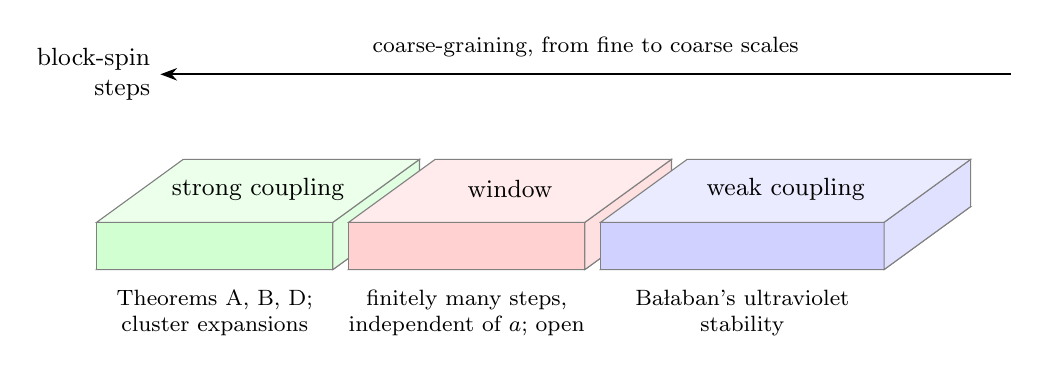
\begin{tikzpicture}[x={(1cm,0cm)},y={(0.55cm,0.4cm)},z={(0cm,1cm)}]
% three slabs in perspective
\foreach \x/\w/\c/\t in {0/3/green/{strong coupling},3.2/3/red/{window},6.4/3.6/blue/{weak coupling}}{
  \filldraw[fill=\c!25,draw=black!50] (\x,0,0)--(\x+\w,0,0)--(\x+\w,2,0)--(\x,2,0)--cycle;
  \filldraw[fill=\c!18,draw=black!50] (\x,0,0)--(\x+\w,0,0)--(\x+\w,0,0.6)--(\x,0,0.6)--cycle;
  \filldraw[fill=\c!12,draw=black!50] (\x+\w,0,0)--(\x+\w,2,0)--(\x+\w,2,0.6)--(\x+\w,0,0.6)--cycle;
  \filldraw[fill=\c!8,draw=black!50] (\x,0,0.6)--(\x+\w,0,0.6)--(\x+\w,2,0.6)--(\x,2,0.6)--cycle;
  \node[font=\small] at (\x+\w/2,1,0.62) {\t};
}
\node[font=\footnotesize,align=center] at (1.5,0,-0.55) {Theorems A, B, D;\\ cluster expansions};
\node[font=\footnotesize,align=center] at (4.7,0,-0.55) {finitely many steps,\\ independent of $a$; open};
\node[font=\footnotesize,align=center] at (8.2,0,-0.55) {Ba{\l}aban's ultraviolet\\ stability};
\draw[-{Stealth[length=6pt]},thick] (10.4,2.2,1.6)--(-0.4,2.2,1.6) node[left,font=\small,align=right]{block-spin\\ steps};
\node[font=\footnotesize] at (5,2.2,1.95) {coarse-graining, from fine to coarse scales};
\end{tikzpicture}
\end{document}
